\documentclass[landscape,10pt]{article}
\usepackage[utf8]{inputenc}
\usepackage[dvipsnames]{xcolor}
\usepackage{tikz}
\usepackage{geometry}
\geometry{a4paper, margin=0.5cm}

% Definition der Schalenfarben
\definecolor{shell2}{RGB}{173, 216, 230} % Zweier-Schale (Mesonen)
\definecolor{shell3}{RGB}{255, 204, 153} % Dreier-Schale (Quarks)
\definecolor{shell4}{RGB}{144, 238, 144} % Vierer-Schale (Atome)
\definecolor{shell5}{RGB}{255, 182, 193} % Fünfer-Schale (E8/Gold)

\begin{document}
	
	\begin{center}
		\Huge \textbf{\#Energiedoku: Arithmetisches Periodensystem} \\
		\large \textit{Symmetrie-Stufen der Riemannschen Nullstellen-Quadrupel}
	\end{center}
	
	\vspace{1cm}
	
	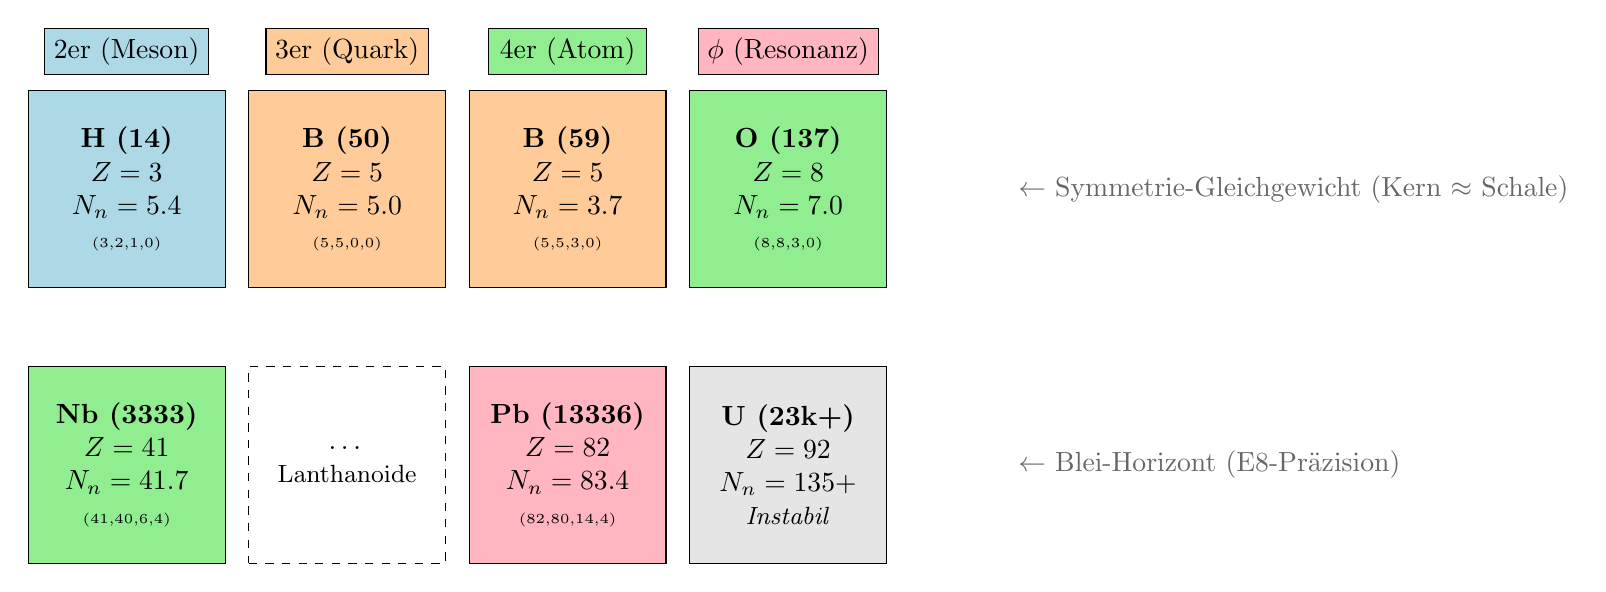
\begin{tikzpicture}[x=2.8cm, y=3.5cm]
		
		% Legende
		\node[draw, fill=shell2, minimum width=2cm] at (0, 0.5) {2er (Meson)};
		\node[draw, fill=shell3, minimum width=2cm] at (1, 0.5) {3er (Quark)};
		\node[draw, fill=shell4, minimum width=2cm] at (2, 0.5) {4er (Atom)};
		\node[draw, fill=shell5, minimum width=2cm] at (3, 0.5) {$\phi$ (Resonanz)};
		
		% --- Reihe 1: Die Fundamente ---
		\node[draw, fill=shell2, minimum height=2.5cm, minimum width=2.5cm, align=center] at (0, 0) 
		{\textbf{H (14)} \\ $Z=3$ \\ $N_n=5.4$ \\ \tiny (3,2,1,0)};
		\node[draw, fill=shell3, minimum height=2.5cm, minimum width=2.5cm, align=center] at (1, 0) 
		{\textbf{B (50)} \\ $Z=5$ \\ $N_n=5.0$ \\ \tiny (5,5,0,0)};
		\node[draw, fill=shell3, minimum height=2.5cm, minimum width=2.5cm, align=center] at (2, 0) 
		{\textbf{B (59)} \\ $Z=5$ \\ $N_n=3.7$ \\ \tiny (5,5,3,0)};
		\node[draw, fill=shell4, minimum height=2.5cm, minimum width=2.5cm, align=center] at (3, 0) 
		{\textbf{O (137)} \\ $Z=8$ \\ $N_n=7.0$ \\ \tiny (8,8,3,0)};
		
		% --- Reihe 2: Die Sättigung ---
		\node[draw, fill=shell4, minimum height=2.5cm, minimum width=2.5cm, align=center] at (0, -1) 
		{\textbf{Nb (3333)} \\ $Z=41$ \\ $N_n=41.7$ \\ \tiny (41,40,6,4)};
		\node[draw, fill=white, draw=black, dashed, minimum height=2.5cm, minimum width=2.5cm, align=center] at (1, -1) 
		{\dots \\ \small Lanthanoide};
		\node[draw, fill=shell5, minimum height=2.5cm, minimum width=2.5cm, align=center] at (2, -1) 
		{\textbf{Pb (13336)} \\ $Z=82$ \\ $N_n=83.4$ \\ \tiny (82,80,14,4)};
		
		% --- Reihe 3: Transurane (Jenseits von E8-Sättigung) ---
		\node[draw, fill=gray!20, minimum height=2.5cm, minimum width=2.5cm, align=center] at (3, -1) 
		{\textbf{U (23k+)} \\ $Z=92$ \\ $N_n=135+$ \\ \small \textit{Instabil}};
		
		% Anmerkungen am Rand
		\node[anchor=west, text=black!60] at (4, 0) {$\leftarrow$ Symmetrie-Gleichgewicht (Kern $\approx$ Schale)};
		\node[anchor=west, text=black!60] at (4, -1) {$\leftarrow$ Blei-Horizont (E8-Präzision)};
		
	\end{tikzpicture}
	
	\vspace{1cm}
	
	\textbf{Erläuterung der Karte:}
	\begin{itemize}
		\item \textbf{Z (Protonen):} Entspricht dem Skalar-Wert $e$ des Prim-Quaternions.
		\item \textbf{$N_n$ (Neutronen):} Der arithmetische Puffer $Z \cdot (Kern/Schale)$.
		\item \textbf{Status:} Farbcodes zeigen die Schalendominanz. Bei 3333 erreichen wir die "Goldene Ordnung" ($\phi$).
		\item \textbf{Transurane:} Jenseits von $N=13336$ bricht die 4er-Raumzeit-Struktur zugunsten reiner E8-Vakuum-Energie auf.
	\end{itemize}
	
\end{document}